\subsection{Polarized Proton Collisions}

DIS is an electromagnetic process, so the techniques used to study the polarized gluon distribution in that environment must rely on higher-order QCD effects. In contrast, collisions of polarized protons are usually mediated by the strong force. Spin-dependent observables in these collisions are  directly sensitive to the polarized gluon content, as a significant fraction of hard scatterings contain one or more gluons in the initial partonic state. A given observable's particular sensitivity to polarized glue is calculable thanks to the triumvirate of asymptotic freedom, factorization, and PDF universality.  As of this writing, calculations performed at next-to-leading order (NLO) are the state of the art.

\begin{figure}\begin{center}
  \includegraphics[width=0.5\textwidth]{figures/partonic_asymmetry}
  \caption{Lowest-order analyzing powers for various partonic subprocesses
  present in polarized proton collisions \cite{Bunce:2000uv}.}
  \label{fig:partonic-asymmetries}
\end{center}\end{figure}

In principle one could directly measure a polarized cross section, e.g. a polarized analogue to \ref{eqn:factorization}.  In practice, a more precise result is obtained through asymmetry measurements that use the ratio of polarized and unpolarized cross sections to cancel out several sources of spin-independent uncertainty present in the absolute cross section measurements.  The observable of primary interest in this work is \(A_{LL}\), defined for inclusive pion production as
%
\begin{equation}
  A_{LL}(\pi + X) = \sum_{a,b,c} \frac{\Delta f_a(x_A, Q^2) \otimes \Delta f_b(x_B, Q^2) \otimes \left[ \hat{a}_{LL}^{ab \rightarrow cX} \sigma_{ab \rightarrow cX} \right] \otimes D_c^{\pi}(z)}{f_a(x_A, Q^2) \otimes f_b(x_B, Q^2) \otimes \sigma_{ab \rightarrow cX} \otimes D_c^{\pi}(z)}.
\end{equation}
%
\(\hat{a}_{LL}^{ab \rightarrow cX} \equiv \Delta \sigma_{ab \rightarrow cX} / \sigma_{ab \rightarrow cX}\) is the asymmetry of the underlying partonic hard scattering.  Figure \ref{fig:partonic-asymmetries} plots partonic asymmetries calculated using perturbative QCD for common subprocesses.  \(A_{LL}\) for charged pion production integrates over all five of these subprocess asymmetries.

\(A_{LL}\) can be measured and interpreted in a perturbative QCD context for a wide variety of final states. This thesis presents results on \(A_{LL}\) for inclusive charged pion production, as well as for charged pions produced azimuthally opposite an identified jet.  Figure \ref{fig:all-predictions} shows the effect of polarized glue on these observables.  The curves represent asymmetries calculated perturbatively at NLO assuming various polarized gluon distributions, ranging from an unpolarized glue (GRSV ZERO) to extreme fully-polarized scenarios (GRSV MIN).  The STD scenario in the GRSV \cite{Gluck:2000dy} set represented a best-fit extraction of polarized structure functions from \(g_1\) evolution data at the time of its release, while Gehrmann and Stirling's ``Set C'' \cite{Gehrmann:1995ag} is a scenario in which gluons are strongly polarized at low \(x\) but the overall integral of the gluon polarization is small thanks to a node in the distribution function.  Finally, the DSSV \cite{deFlorian:2008mr} set of structure functions is the first to incorporate data from measurements of \(A_{LL}\), specifically the inclusive \(\pi^0\) channel at PHENIX and the inclusive jet channel at STAR.  The measurements in this thesis can be included in a future update to the DSSV set and other similar global analyses in order to directly inform our understanding of the polarized gluon distribution.


\begin{figure}
  \subfloat{
    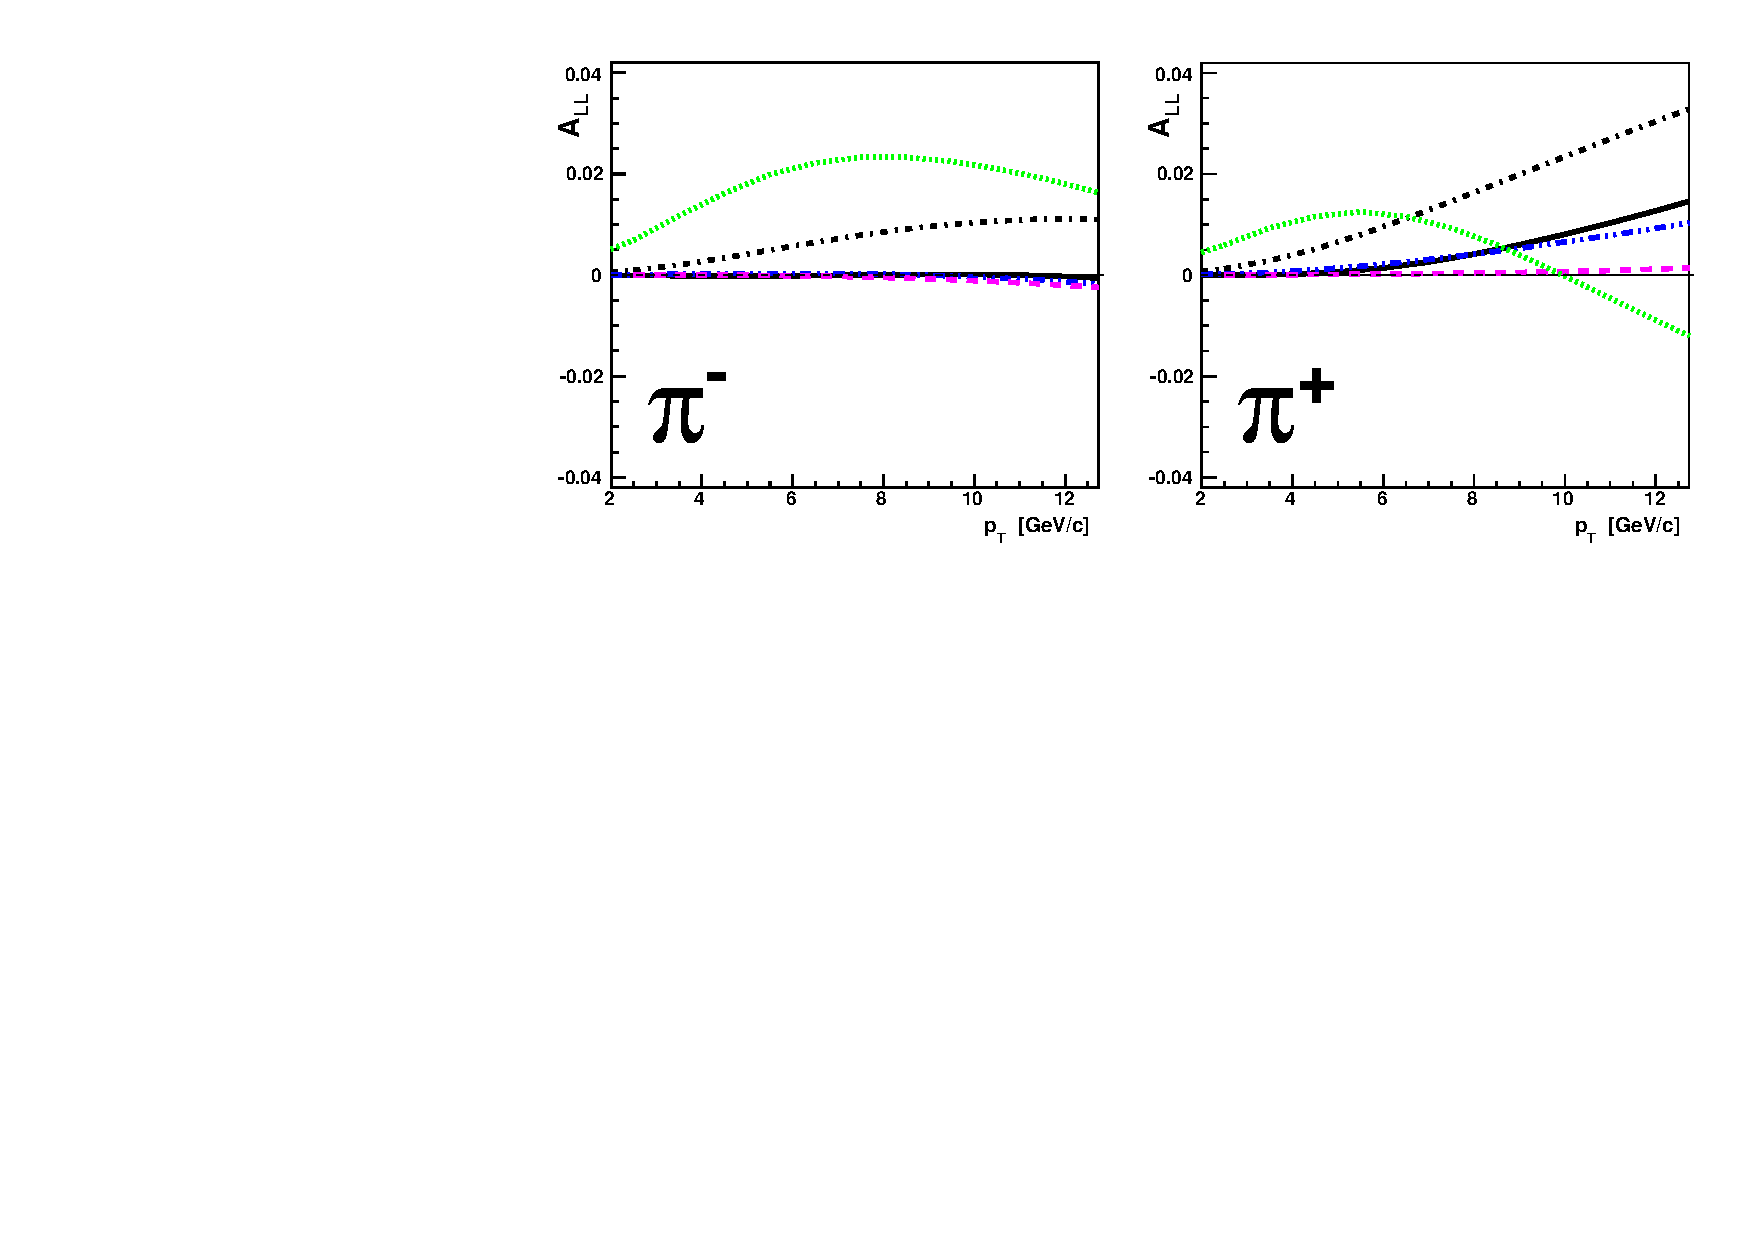
\includegraphics[width=1.0\textwidth]{figures/inclusive_predictions}
  }
  \newline
  \subfloat{
    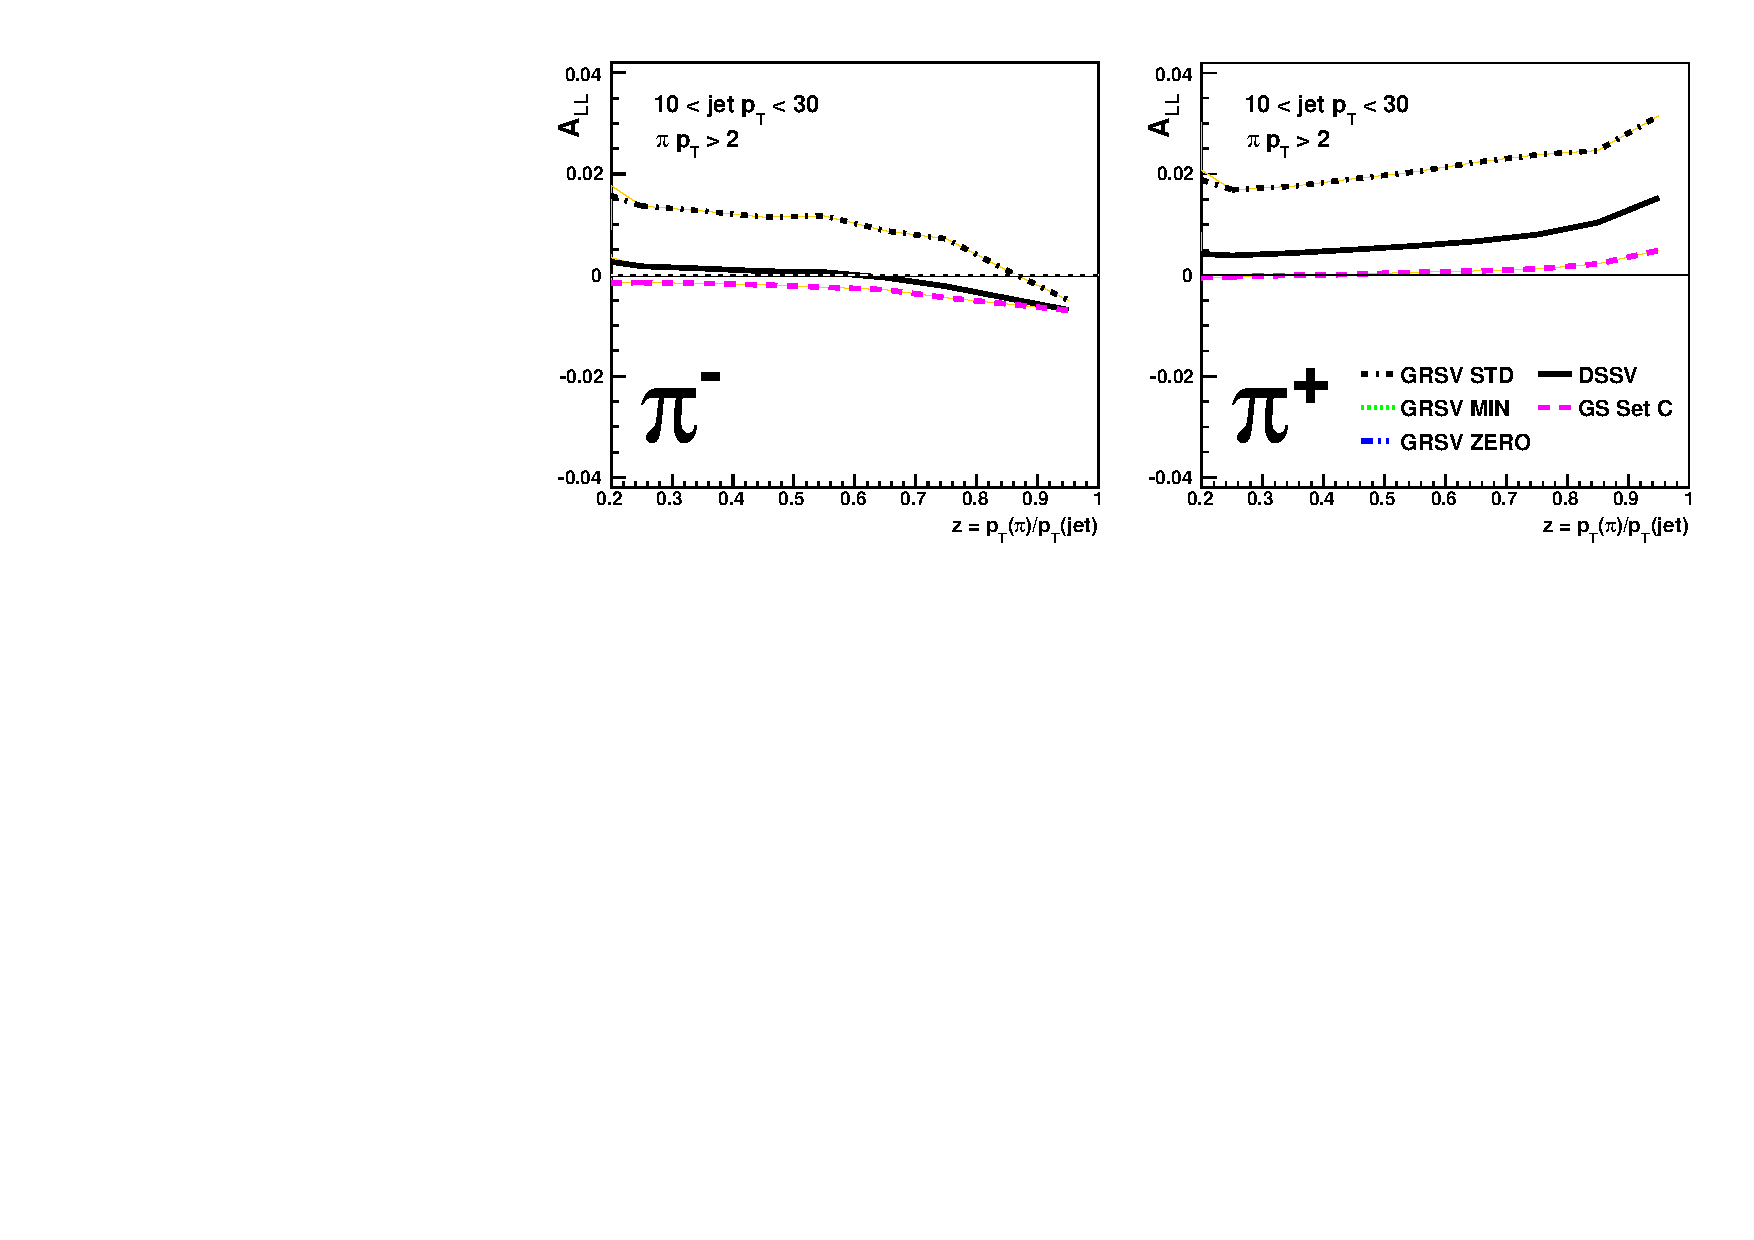
\includegraphics[width=1.0\textwidth]{figures/jet_pion_predictions}
  }
  \caption{Predictions for $A_{LL}$ assuming various input distributions for the gluon polarization \cite{Gluck:2000dy, Gehrmann:1995ag, deFlorian:2008mr}. The pion fragmentation functions can be found in \cite{deFlorian:2007nk}, and the NLO calculation was performed in the purely inclusive case by J\"ager et al. \cite{Jager:2002xm}, and in the jet + pion case by de Florian \cite{deFlorian:2009fw}.}
  \label{fig:all-predictions}
\end{figure}
